\documentclass{article}
% Use with [notoc] option to hide table of contents
\usepackage{../typesetting/styles/note-zh}
% Default shows table of contents
% \usepackage{../styles/note-zh}
\usepackage{bookmark}

\title{AI工具 - 基础使用}
\author{xjh}

\begin{document}

\maketitle

\section{引言: What is AI}
大型语言模型(Large Language Models,简称LLM)是当前人工智能领域最为瞩目的技术之一,它们正在迅速改变我们与计算机交互的方式。本章节将介绍LLM的基本概念、能力范围及其局限性,帮助读者更好地理解和使用这些AI工具。

\subsection{什么是大型语言模型}
大型语言模型是一种基于深度学习的自然语言处理系统,通过在海量文本数据上训练,学习语言的模式、规律和知识。这些模型通常包含数十亿甚至数千亿个参数,使其能够理解、生成和翻译人类语言。

\textcolor{red}{定义:}大型语言模型是一类能够处理和生成自然语言的神经网络模型,它们通过``预训练+微调"的方式,学习语言的统计规律和知识表示。(此处我们将不同的格式数据,如:图片音频,编码成统一格式,输入到大模型中,此时起将具备处理\blue{多模态}数据的能力,如:图像+文本,音频+文本等)

举例来说,如果我们把LLM比作一个学生,那么:
\begin{itemize}
  \item 预训练阶段相当于这个学生阅读了人类历史上的大部分书籍和文章,多为大公司开发,需要大量计算资源
  \item 微调阶段则相当于针对特定考试进行的专项训练,小公司或个人可以使用开源模型进行微调,适合特定任务
\end{itemize}

\subsection{LLM能做什么}
现代LLM展现出了令人惊叹的多种能力:

\begin{itemize}
  \item \textcolor{blue}{文本生成}:可以撰写文章、故事、诗歌,甚至是代码
  \item \textcolor{blue}{问答系统}:回答各类知识性问题,提供信息和解释
  \item \textcolor{blue}{语言翻译}:在不同语言之间进行翻译
  \item \textcolor{blue}{摘要生成}:将长文本压缩为简短的摘要
  \item \textcolor{blue}{创意写作}:按照指定风格或要求创作内容
  \item \textcolor{blue}{代码辅助}:帮助程序员编写、解释和调试代码
\end{itemize}

\colorbox{yellow}{案例:}当你向ChatGPT询问"如何制作披萨"时,它能够提供从准备材料到烘烤的详细步骤,这是因为模型已经从大量烹饪文本中学习到了相关知识。

\subsection{LLM的局限性}
尽管功能强大,LLM仍有明显的局限:

\begin{itemize}
  \item \textbf{知识截止点}:模型只知道训练数据中的信息,对于训练后发生的事件一无所知,\textcolor{red}{通过添加search的功能来缓解}
  \item \textbf{事实性问题}:有时会生成看似可信但实际不准确的内容(``幻觉"现象),\textcolor{red}{需要人工审核}
  \item \textbf{计算能力有限}:无法执行复杂的数学计算或推理
  \item \textbf{上下文窗口限制}:一次只能处理有限长度的文本, \textcolor{red}{需要大问题分解小问题,分段处理}
\end{itemize}

\colorbox{yellow}{真实案例:}某用户询问ChatGPT``2023年奥斯卡最佳影片是什么",如果模型的训练数据截止于2022年,它可能会回答``我的知识截止到2022年,无法提供2023年的奥斯卡获奖信息"或者错误地猜测一个答案。

\subsection{如何有效使用LLM}
了解LLM的能力和局限后,我们可以更有效地使用它:

\begin{itemize}
  \item 提供清晰、具体的指令
  \item 对关键事实信息进行验证
  \item 将LLM作为思考和创作的辅助工具,而非完全依赖
  \item 通过迭代优化提示(prompt)来获得更好的结果
\end{itemize}

\begin{center}
  {\LARGE  \red{LLM(AI)做加法$+$,我们审核做减法$-$}}
\end{center}

\newpage

\section{准备:Where to use AI}
截至2025年4月,国内AI大模型厂商已形成梯队分布,各有专长与市场定位。以下是按综合服务能力、技术实力和应用场景覆盖范围的评估排名。

\begin{table}[htbp]
  \centering
  \begin{tabular}{|p{3cm}|p{12cm}|}
    \hline
    \textbf{厂商} & \textbf{核心能力与特点} \\
    \hline
    百度-文心一言 &
    \begin{itemize}
      \item 参数规模2600亿,覆盖搜索、智能驾驶等场景
      \item 日均调用量超10亿次,支持多模态生成
      \item 开源策略推动行业生态发展
      \item 官网:\url{https://wenxin.baidu.com}
    \end{itemize} \\
    \hline
    阿里云-通义千问 &
    \begin{itemize}
      \item 千亿级参数MoE架构,支持文本/图像/视频生成
      \item 政务/金融市占率超40\%,开源模型下载量破1.8亿
      \item 企业级服务闭环完善
      \item 官网:\url{https://tongyi.aliyun.com}
    \end{itemize} \\
    \hline
    腾讯-混元大模型 &
    \begin{itemize}
      \item 万亿级参数,深度集成微信生态(DAU超3亿)
      \item 游戏AI工具链降本70\%,支持多模态理解与任务执行
      \item 官网:\url{https://hunyuan.tencent.com}
    \end{itemize} \\
    \hline
  \end{tabular}
  \caption{第一类大模型厂商,\red{大而全}}
\end{table}

\begin{table}[htbp]
  \centering
  \begin{tabular}{|p{3cm}|p{12cm}|}
    \hline
    \textbf{厂商} & \textbf{核心能力与特点} \\
    \hline
    华为-盘古大模型 \\ \red{偏工业应用,个人使用有门槛} &
    \begin{itemize}
      \item 行业大模型适配矿山/气象/医药场景
      \item 端云协同架构降低30\%推理成本
      \item 昇腾AI集群算力全球前三
      \item 官网:\url{https://www.huaweicloud.com/product/pangu}
    \end{itemize} \\
    \hline
    商汤科技-日日新 &
    \begin{itemize}
      \item 多模态生成工具日均创作超百万次
      \item 影视/广告行业覆盖率超60\%
      \item 视频生成时序一致性技术领先
      \item 官网:\url{https://www.sensetime.com}
    \end{itemize} \\
    \hline
    科大讯飞 \\ 星火大模型 &
    \begin{itemize}
      \item 教育题库生成准确率98\%
      \item 医疗诊断覆盖3万家医院
      \item 国产化训练框架适配昇腾芯片
      \item 官网:\url{https://xinghuo.xfyun.cn}
    \end{itemize} \\
    \hline
  \end{tabular}
  \caption{第二类大模型厂商,\red{工业应用}}
\end{table}

\begin{table}[htbp]
  \centering
  \begin{tabular}{|p{3cm}|p{12cm}|}
    \hline
    \textbf{厂商} & \textbf{核心能力与特点} \\
    \hline
    DeepSeek(深度求索) &
    \begin{itemize}
      \item 开源生态快速扩张
      \item 推理成本低至GPT-4o的1/10
      \item 专业领域(科技/金融)表现媲美国际顶尖模型
      \item 官网:\url{https://www.deepseek.com}
    \end{itemize} \\
    \hline
    智谱AI-智谱清言 &
    \begin{itemize}
      \item 知识图谱构建能力突出
      \item 开源GLM-4B社区开发者超10万
      \item 代码生成能力达GPT-4水平
      \item 官网:\url{https://chatglm.cn}
    \end{itemize} \\
    \hline
    字节跳动 \\ 豆包 &
    \begin{itemize}
      \item 多模态交互能力覆盖抖音/飞书等50+业务
      \item 日均生成短视频超50万条
      \item 推理效率与成本控制领先
      \item 官网:\url{https://www.doubao.com}
    \end{itemize} \\
    \hline
    月之暗面 \\ Moonshot &
    \begin{itemize}
      \item 长文本处理能力突出(支持200万字上下文)
      \item 浏览器插件实现网页划线提问
      \item 适合学术研究场景
      \item 官网:\url{https://www.moonshot.cn}
    \end{itemize} \\
    \hline
  \end{tabular}
  \caption{第三类大模型厂商,有\red{突出业务}}
\end{table}

\newpage
\section{使用:How to use AI}

\red{通用使用逻辑:} 使用提示词(prompt)和系统提示词(system prompt)作为输入,LLM会根据这些提示生成相应的输出。\textbf{提示词(Prompt)}:用户输入的具体问题或请求,可以是文本、图片、音频等多种形式。\textbf{系统提示词(System Prompt)}:用于引导模型生成特定类型输出的提示,如输出ppt格式、word格式和特定语言的代码等。

此处我们用两个任务作为例子,分别是\red{PPT生成}和\red{图片生成}。\blue{目前效果最好的任务为文本生成,图片生成对文字处理较差,PPT生成效果较好。}

\subsection{PPT生成}

\noindent 注:此处我们使用Deepseek \url{https://chat.deepseek.com/} 收集信息, 阿里云 \url{https://tongyi.aliyun.com/aippt}进行PPT生成。  同时 \url{https://kimi.moonshot.cn/kimiplus/conpg18t7lagbbsfqksg}  \url{https://chatglm.cn/main/gdetail/670e3c3e119b48fe5a851149} 等提供文本转PPT的厂商也可以使用。

生成逻辑:提出我们的问题,我们使用《衡阳师范学院校史》为例,第一步,收集信息,我们需要生成一个含有校史的结构性文本,此时我们可以使用联网搜索的功能,获取到足够详细的信息$A$。第二步,将$A$作为输入,给具有PPT生成功能的模型进行处理,生成最终的PPT文件。(对于有些平台,不需要我们提供$A$,直接输入问题即可,但其内部还是生成$A$。)

\subsubsection{步骤1:收集信息}\label{sec:collect_info}

图\ref{fig:collect_info}展示了我们在Deepseek上输入的内容,(选择深度思考和search),模型会联网搜索相关信息并生成结构化文本$A$。图\ref{fig:generate_result}展示了生成的结果。\gray{此处替换Deepseek为其他平台也可以。}
\begin{figure}[htbp]
  \centering
  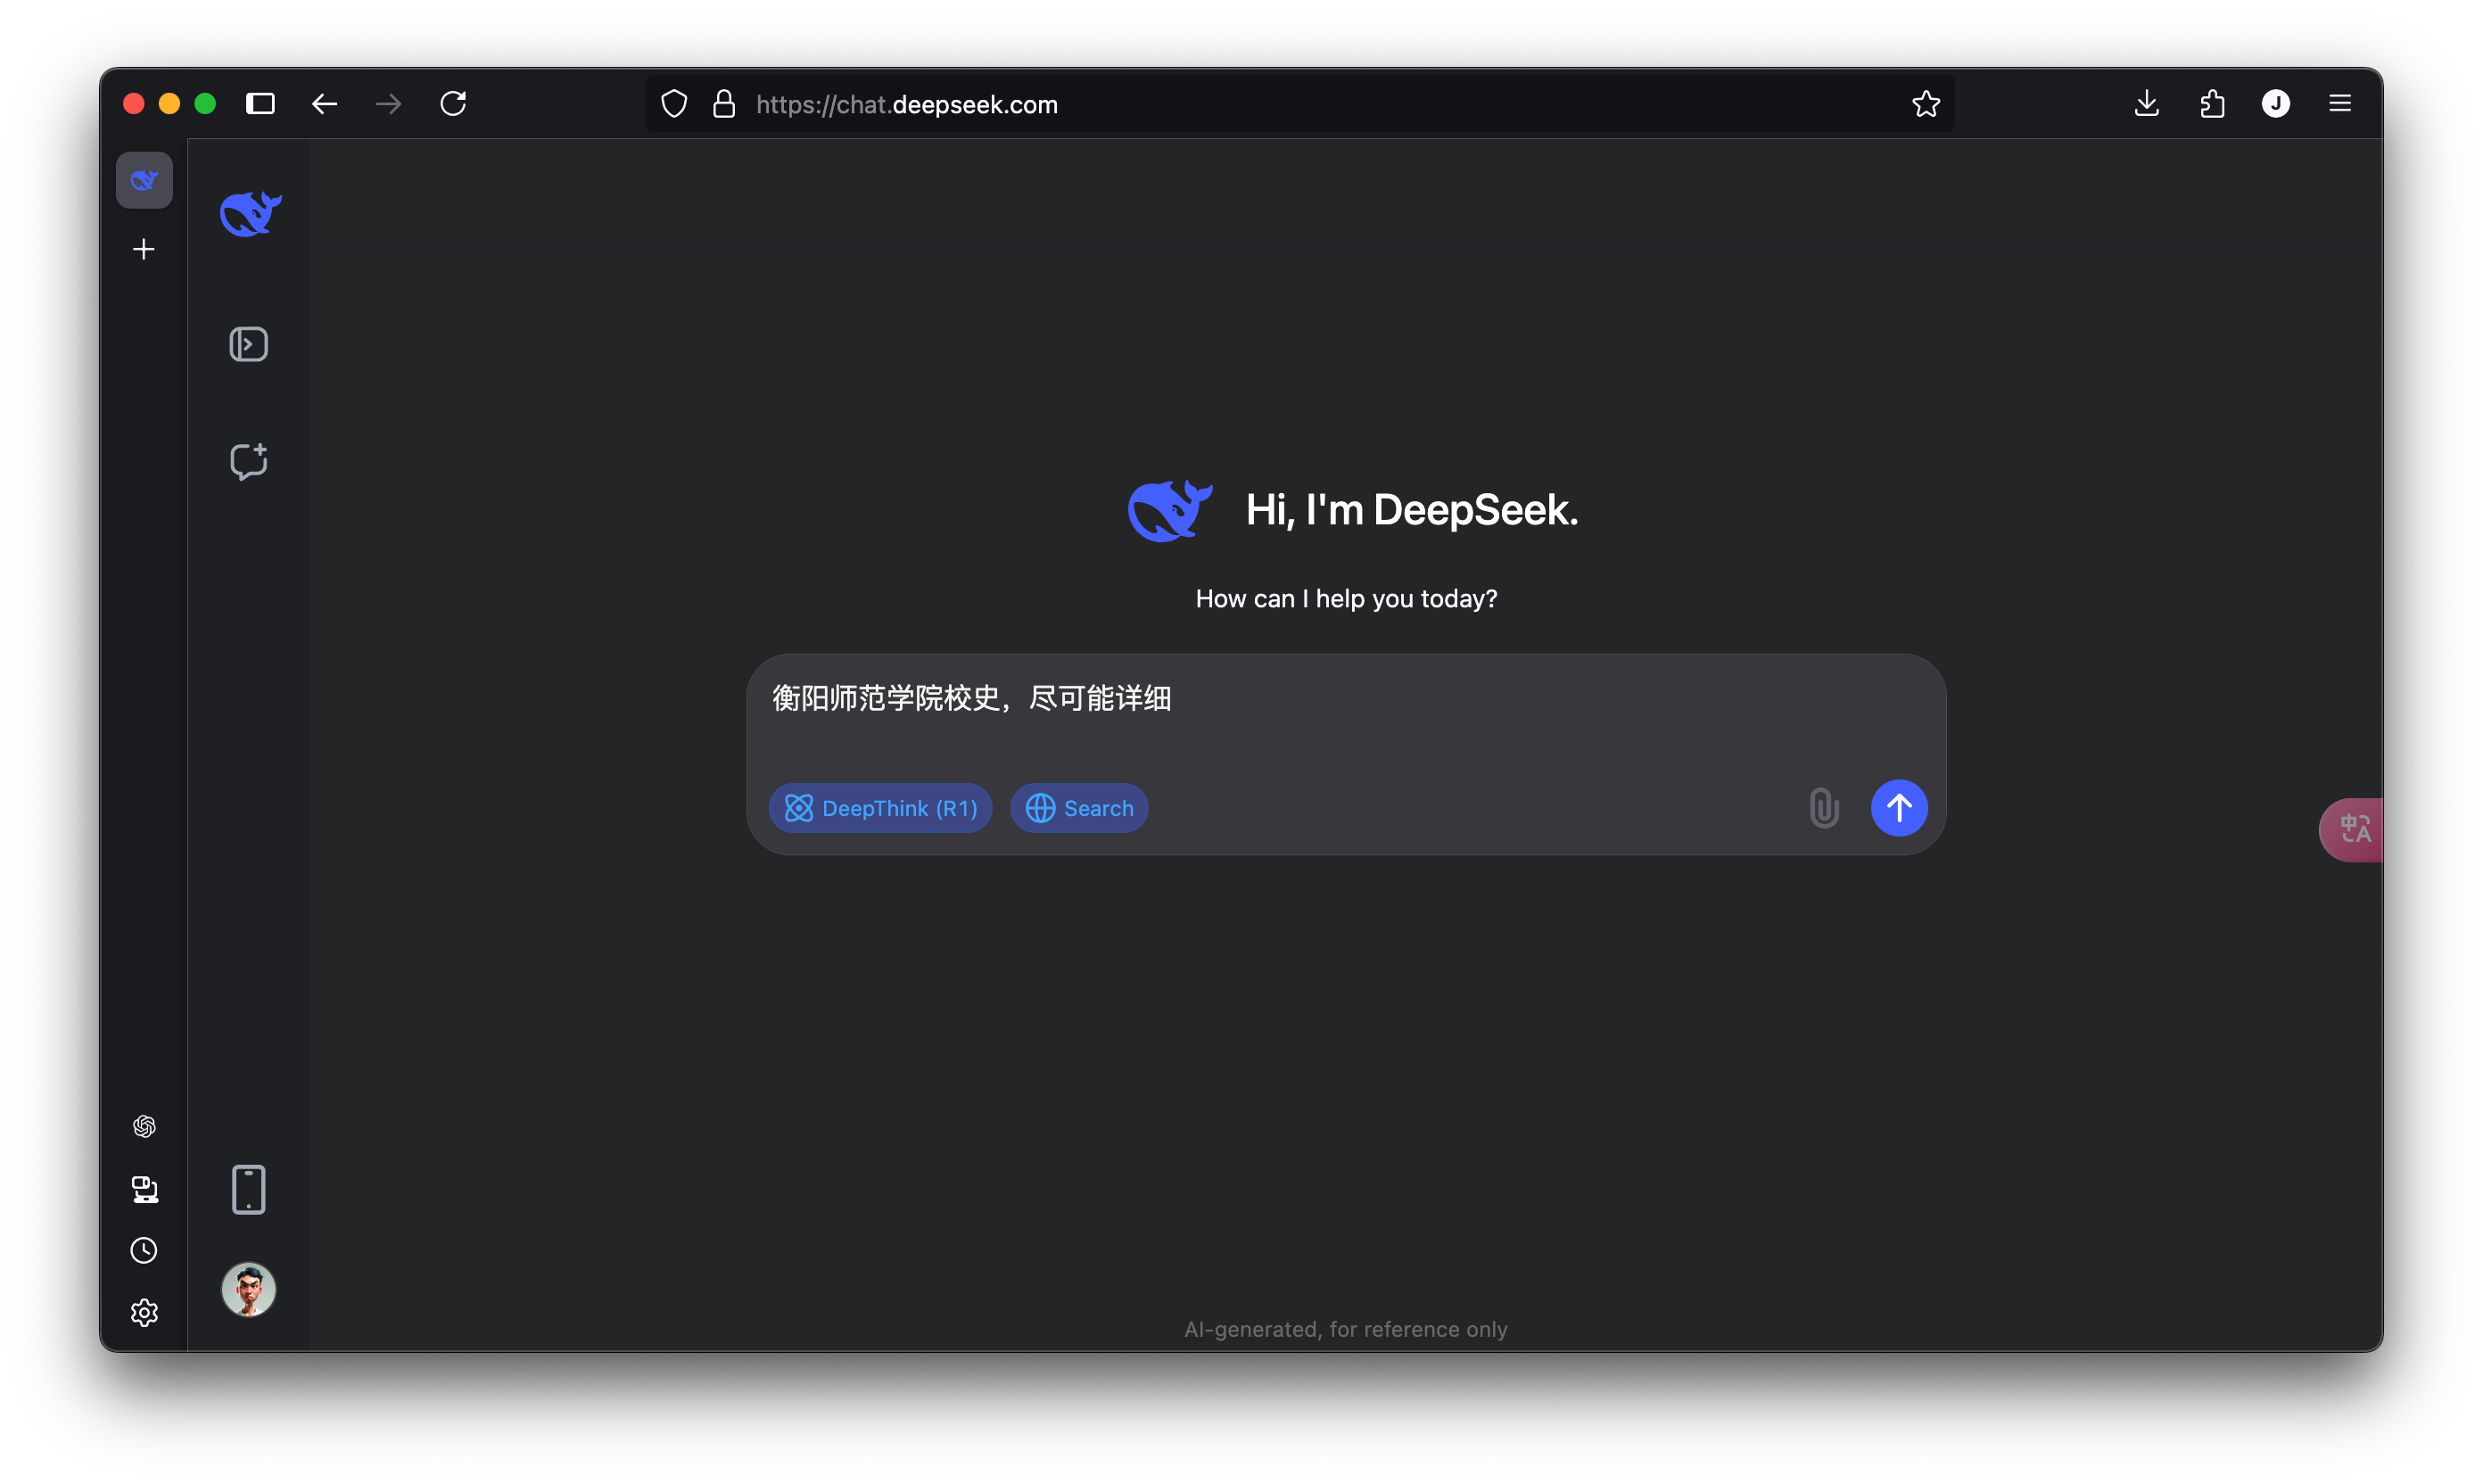
\includegraphics[width=0.8\textwidth]{./fig/search.png}
  \caption{收集信息}
  \label{fig:collect_info}
\end{figure}

\begin{figure}[htbp]
  \centering
  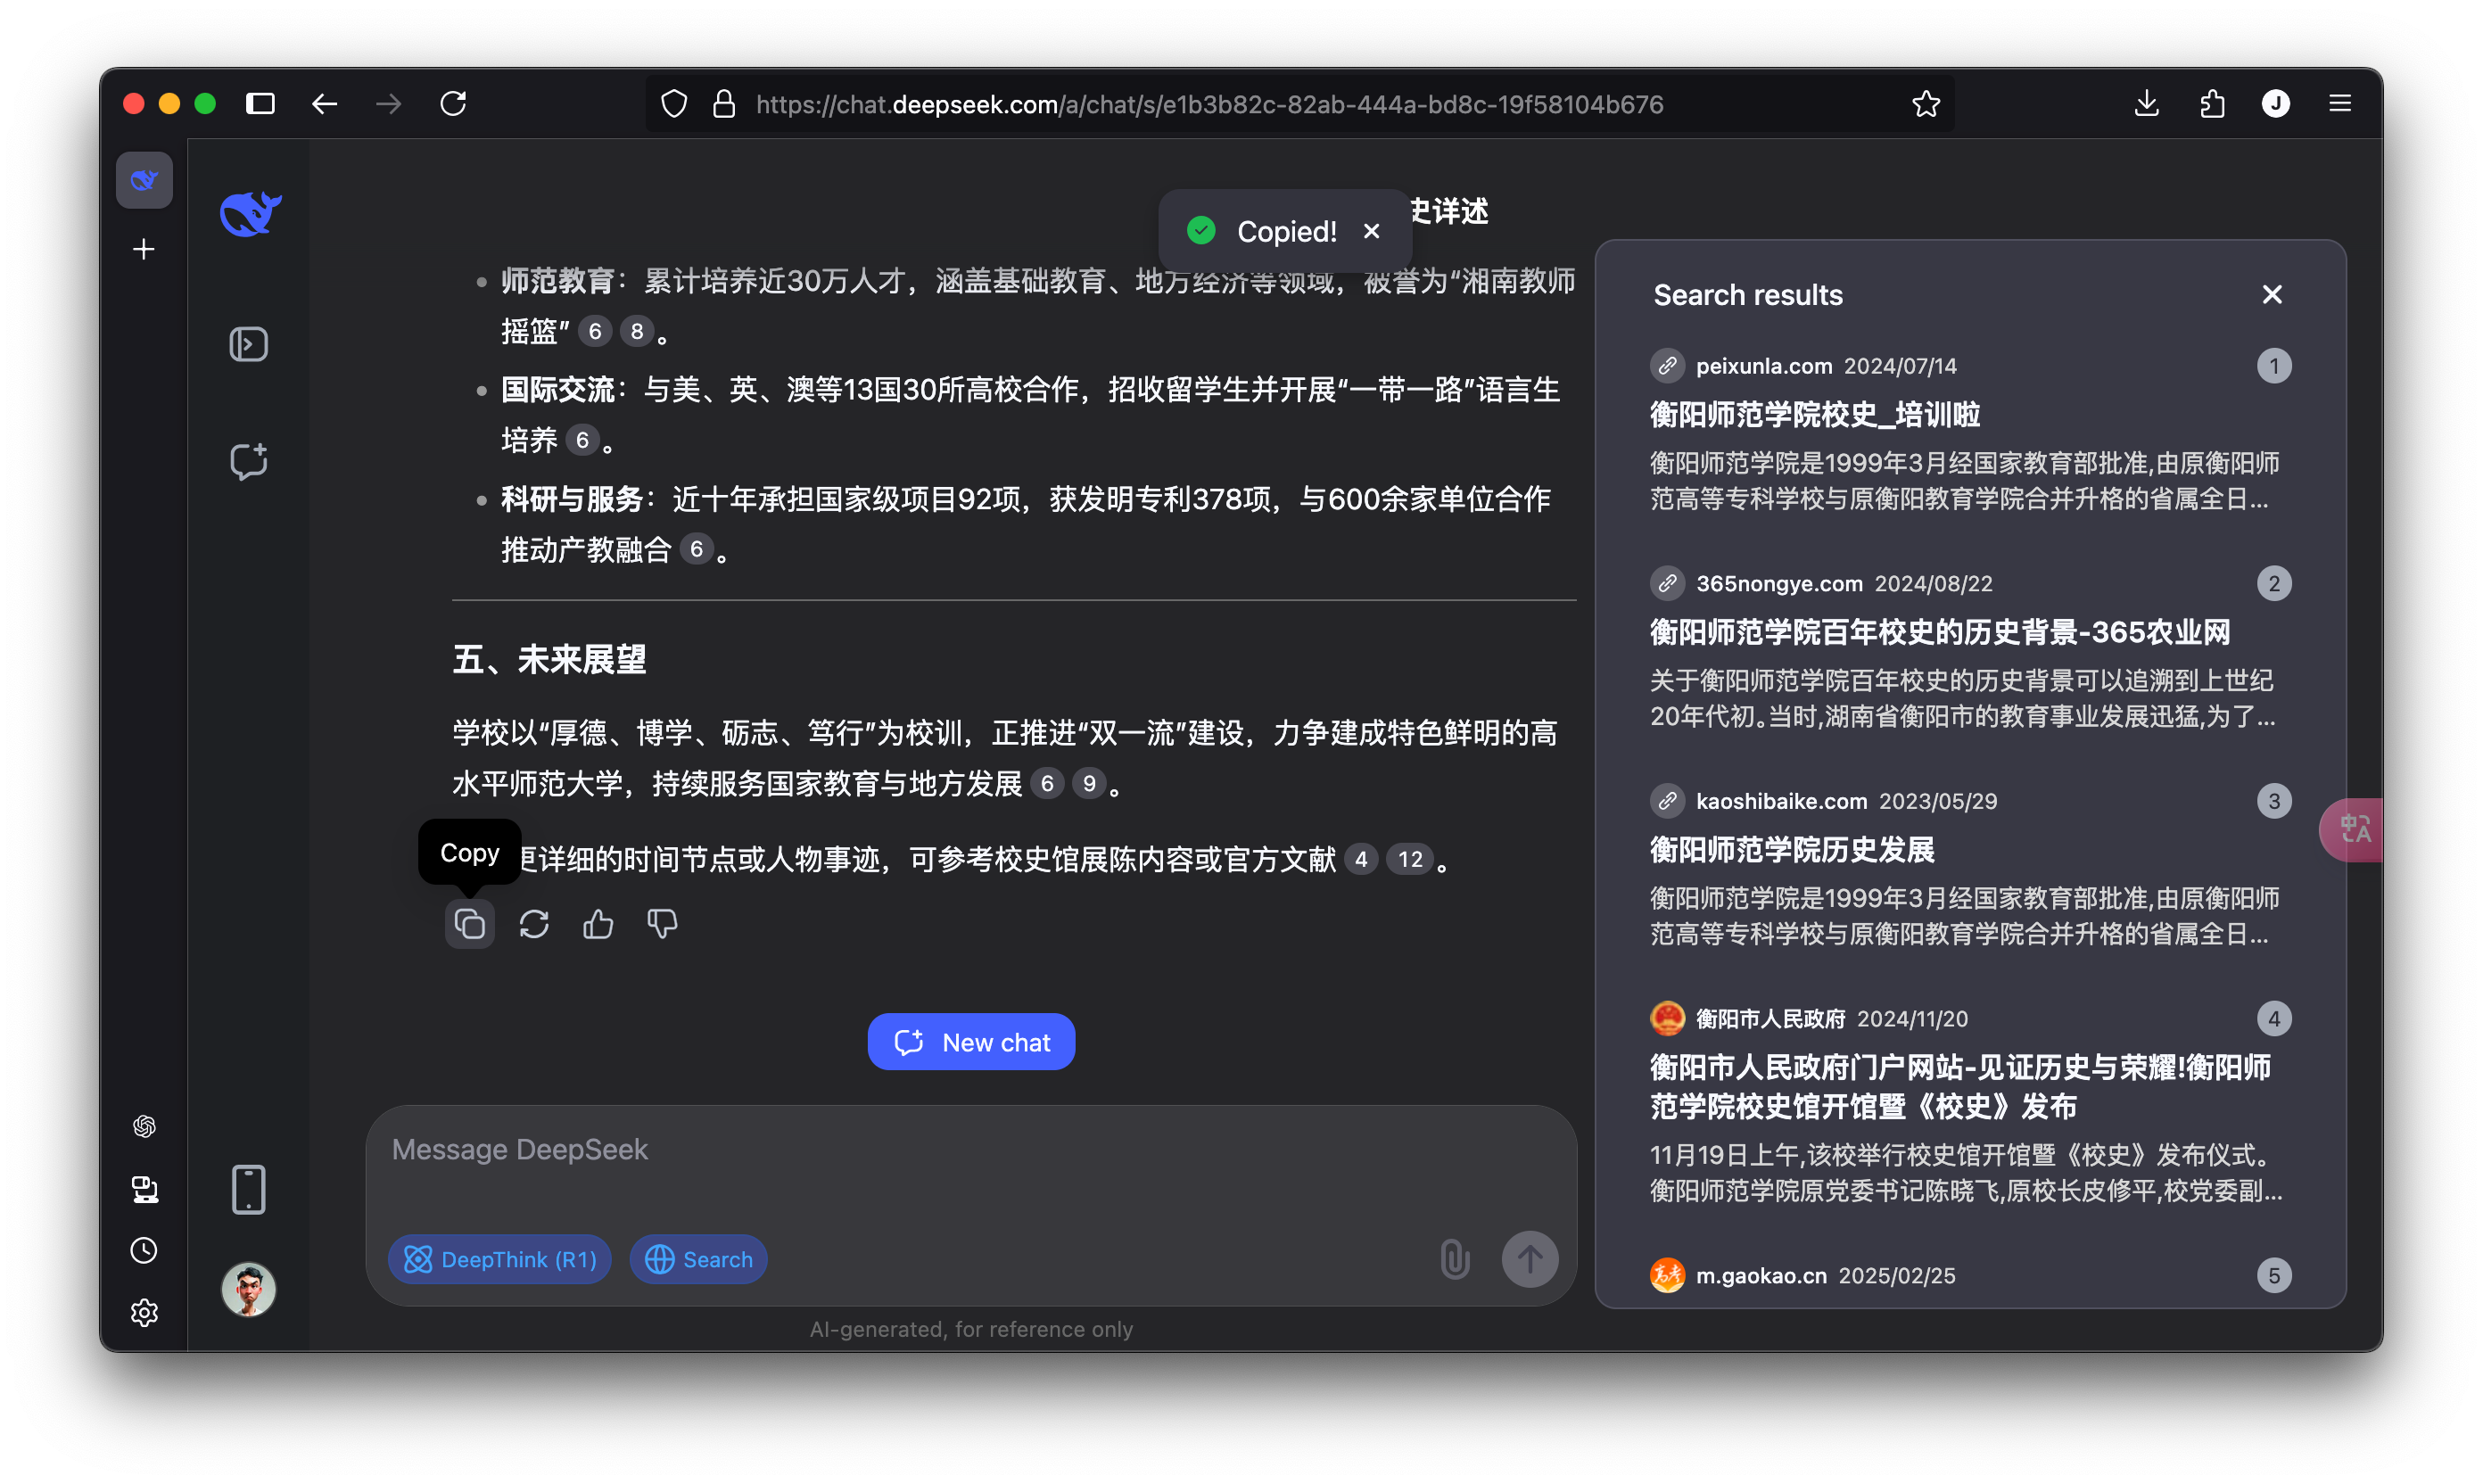
\includegraphics[width=0.8\textwidth]{./fig/search-result.png}
  \caption{生成结果}
  \label{fig:generate_result}
\end{figure}

\subsubsection{步骤2:生成PPT}
图\ref{fig:generate_ppt}展示了我们在阿里云ppt生成模式,先选择ppt模版,模型会根据$A$生成PPT文件。图\ref{fig:generate_ppt}展示了生成的结果。\gray{此处可以替换为其他平台ppt模式。}
\begin{figure}[htbp]
  \centering
  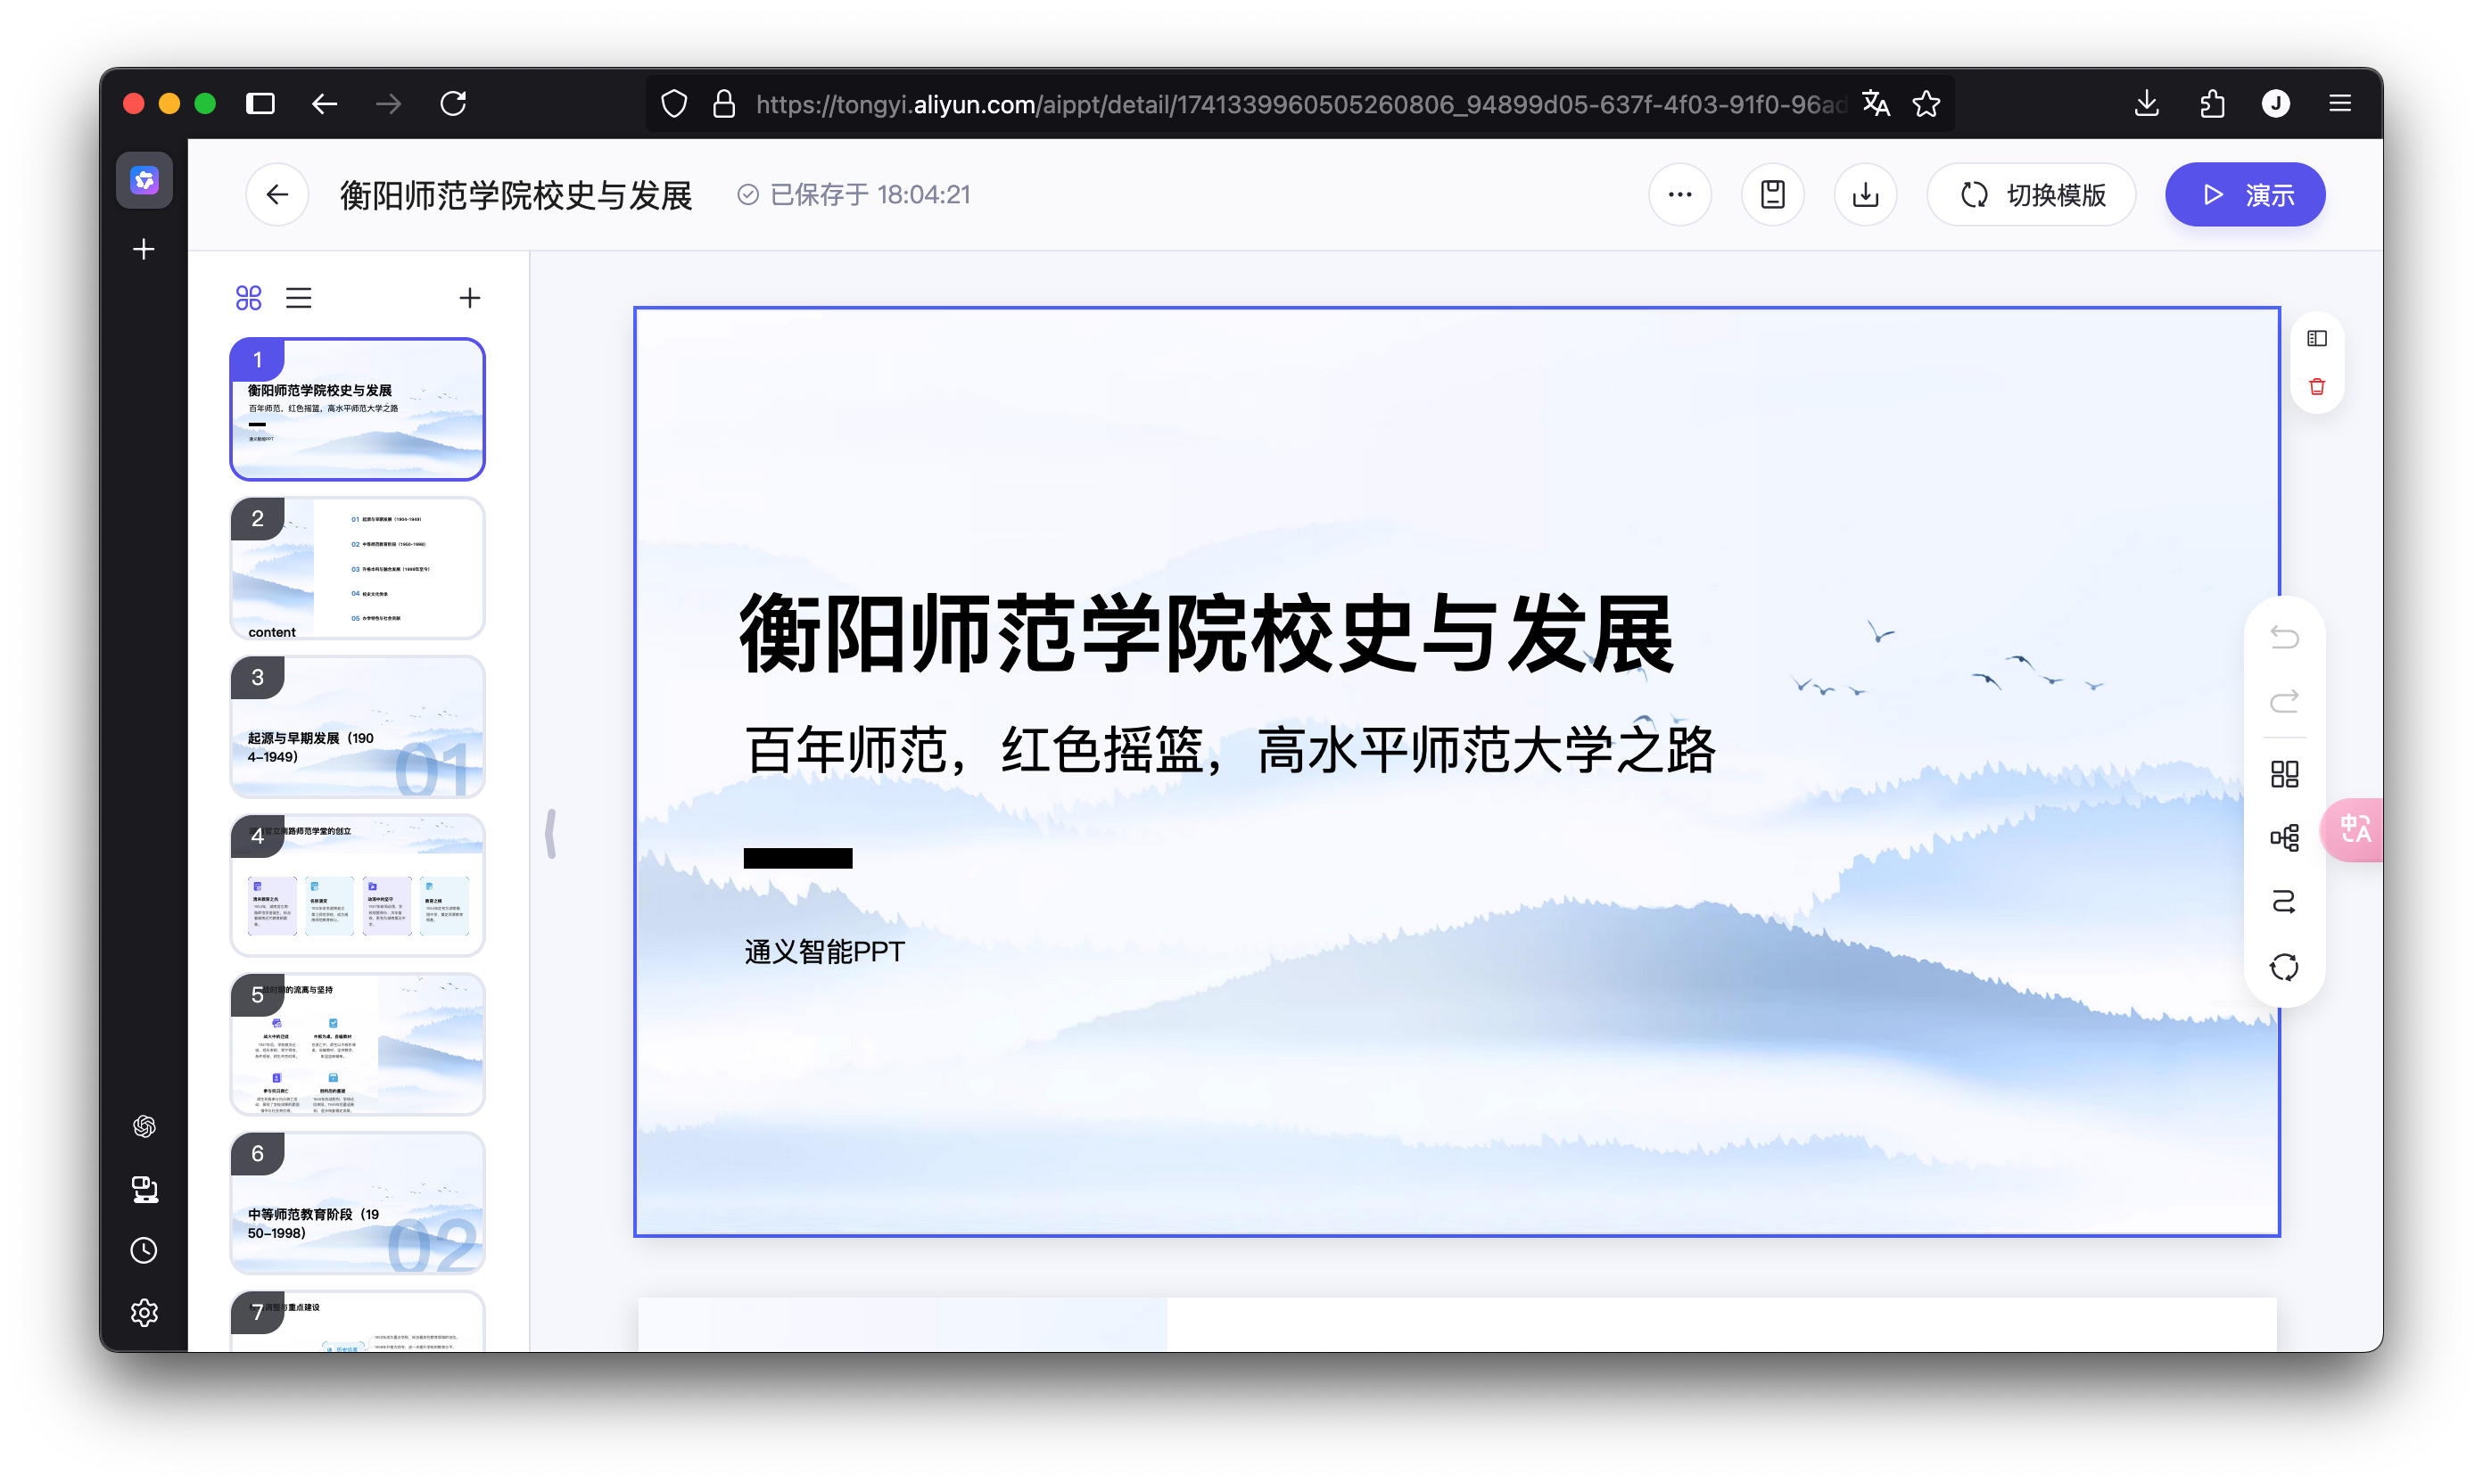
\includegraphics[width=0.7\textwidth]{./fig/ppt.png}
  \caption{生成PPT}
  \label{fig:generate_ppt}
\end{figure}

\subsection{图片生成}

图片生成的方式,我们可以参考\ref{sec:collect_info}的步骤,第一步,收集信息,我们需要生成一个含有图片的结构性文本,此时我们可以使用联网搜索的功能,获取到足够详细的信息$A$。第二步,将$A$作为输入,给具有图片生成功能的模型进行处理,生成最终的图片文件。

我们使用\blue{复古风格的平面设计作品,以衡阳师范学院的标志性建筑为背景,夕阳下的教学楼轮廓在橙色与紫色渐变的天际线中若隐若现,营造出温暖而庄重的氛围。前景中,一位年轻的学生正坐在校园的长椅上,手中捧着一本打开的书,专注地阅读,旁边散落着几片秋叶,象征着知识的沉淀与收获。学生穿着学院的传统制服,蓝白相间的衬衫搭配深蓝色的裤子,胸前佩戴着校徽,展现出学生的自豪与归属感。海报的标题采用手写风格的字体,书写着“梦想起航,未来可期——衡阳师范学院欢迎你”,下方则用更小的字体详细介绍了学院的历史、专业设置以及招生政策。整个设计巧妙融合了学院的文化底蕴与现代教育理念,既体现了学术的严谨,又不失青春的活力。}作为输入,给具有图片生成功能的模型进行处理,生成最终的图片文件。图~\ref{fig:generate_image}展示了我们在\url{https://tongyi.aliyun.com/wanxiang/}阿里通义万象的图片生成的结果。

\begin{figure}[htbp]
  \centering
  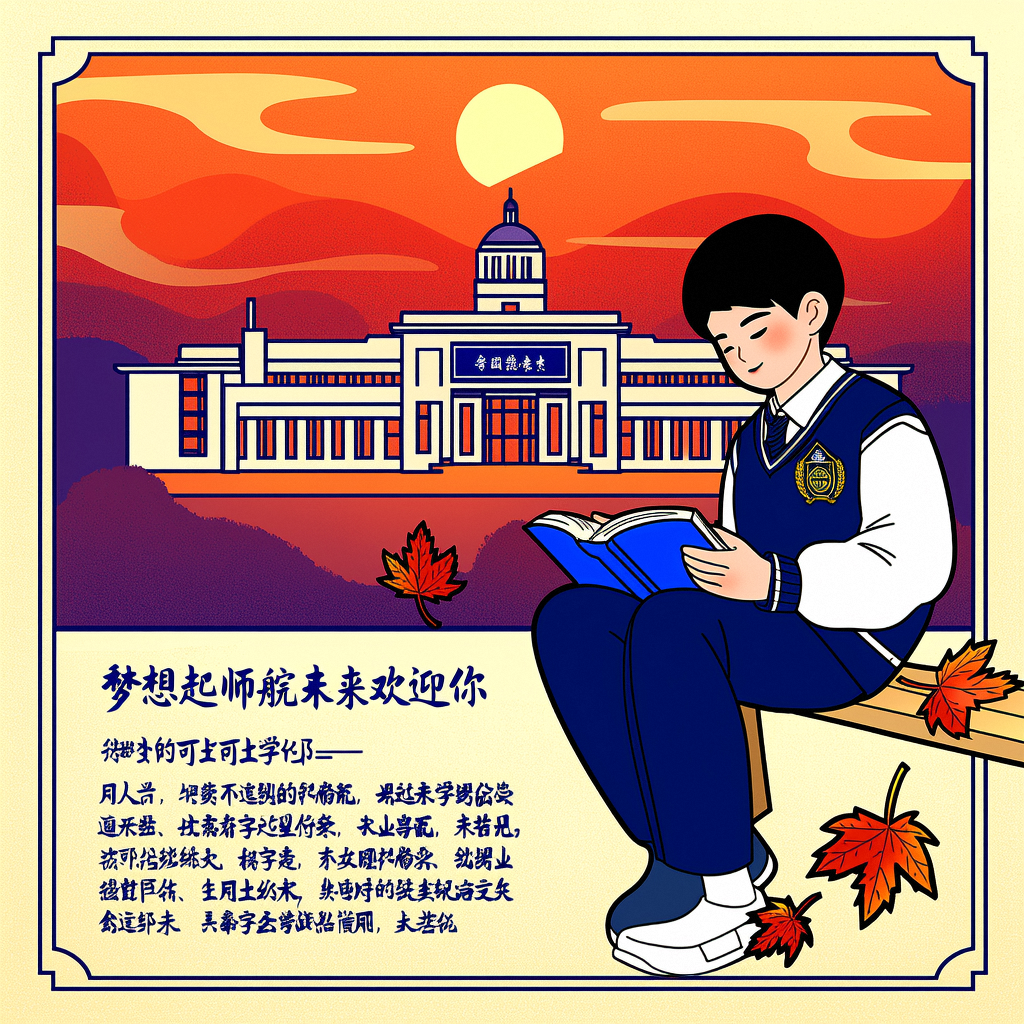
\includegraphics[width=0.7\textwidth]{./fig/image.png}
  \caption{生成图片}
  \label{fig:generate_image}
\end{figure}

从效果上来看,图片的文字是生成的很差的,需要后期调整,由于图像中含有的信息量远大于文本,所以过小的提示词输入,将导致结果很不理想。如果需要产品级的图片,需要引入复杂的模型参数调节,如图~\ref{fig:set_param}所示。我们可以在ComfyUI上进行参数调节。这会较大增加使用的难度。

\begin{figure}[htbp]
  \centering
  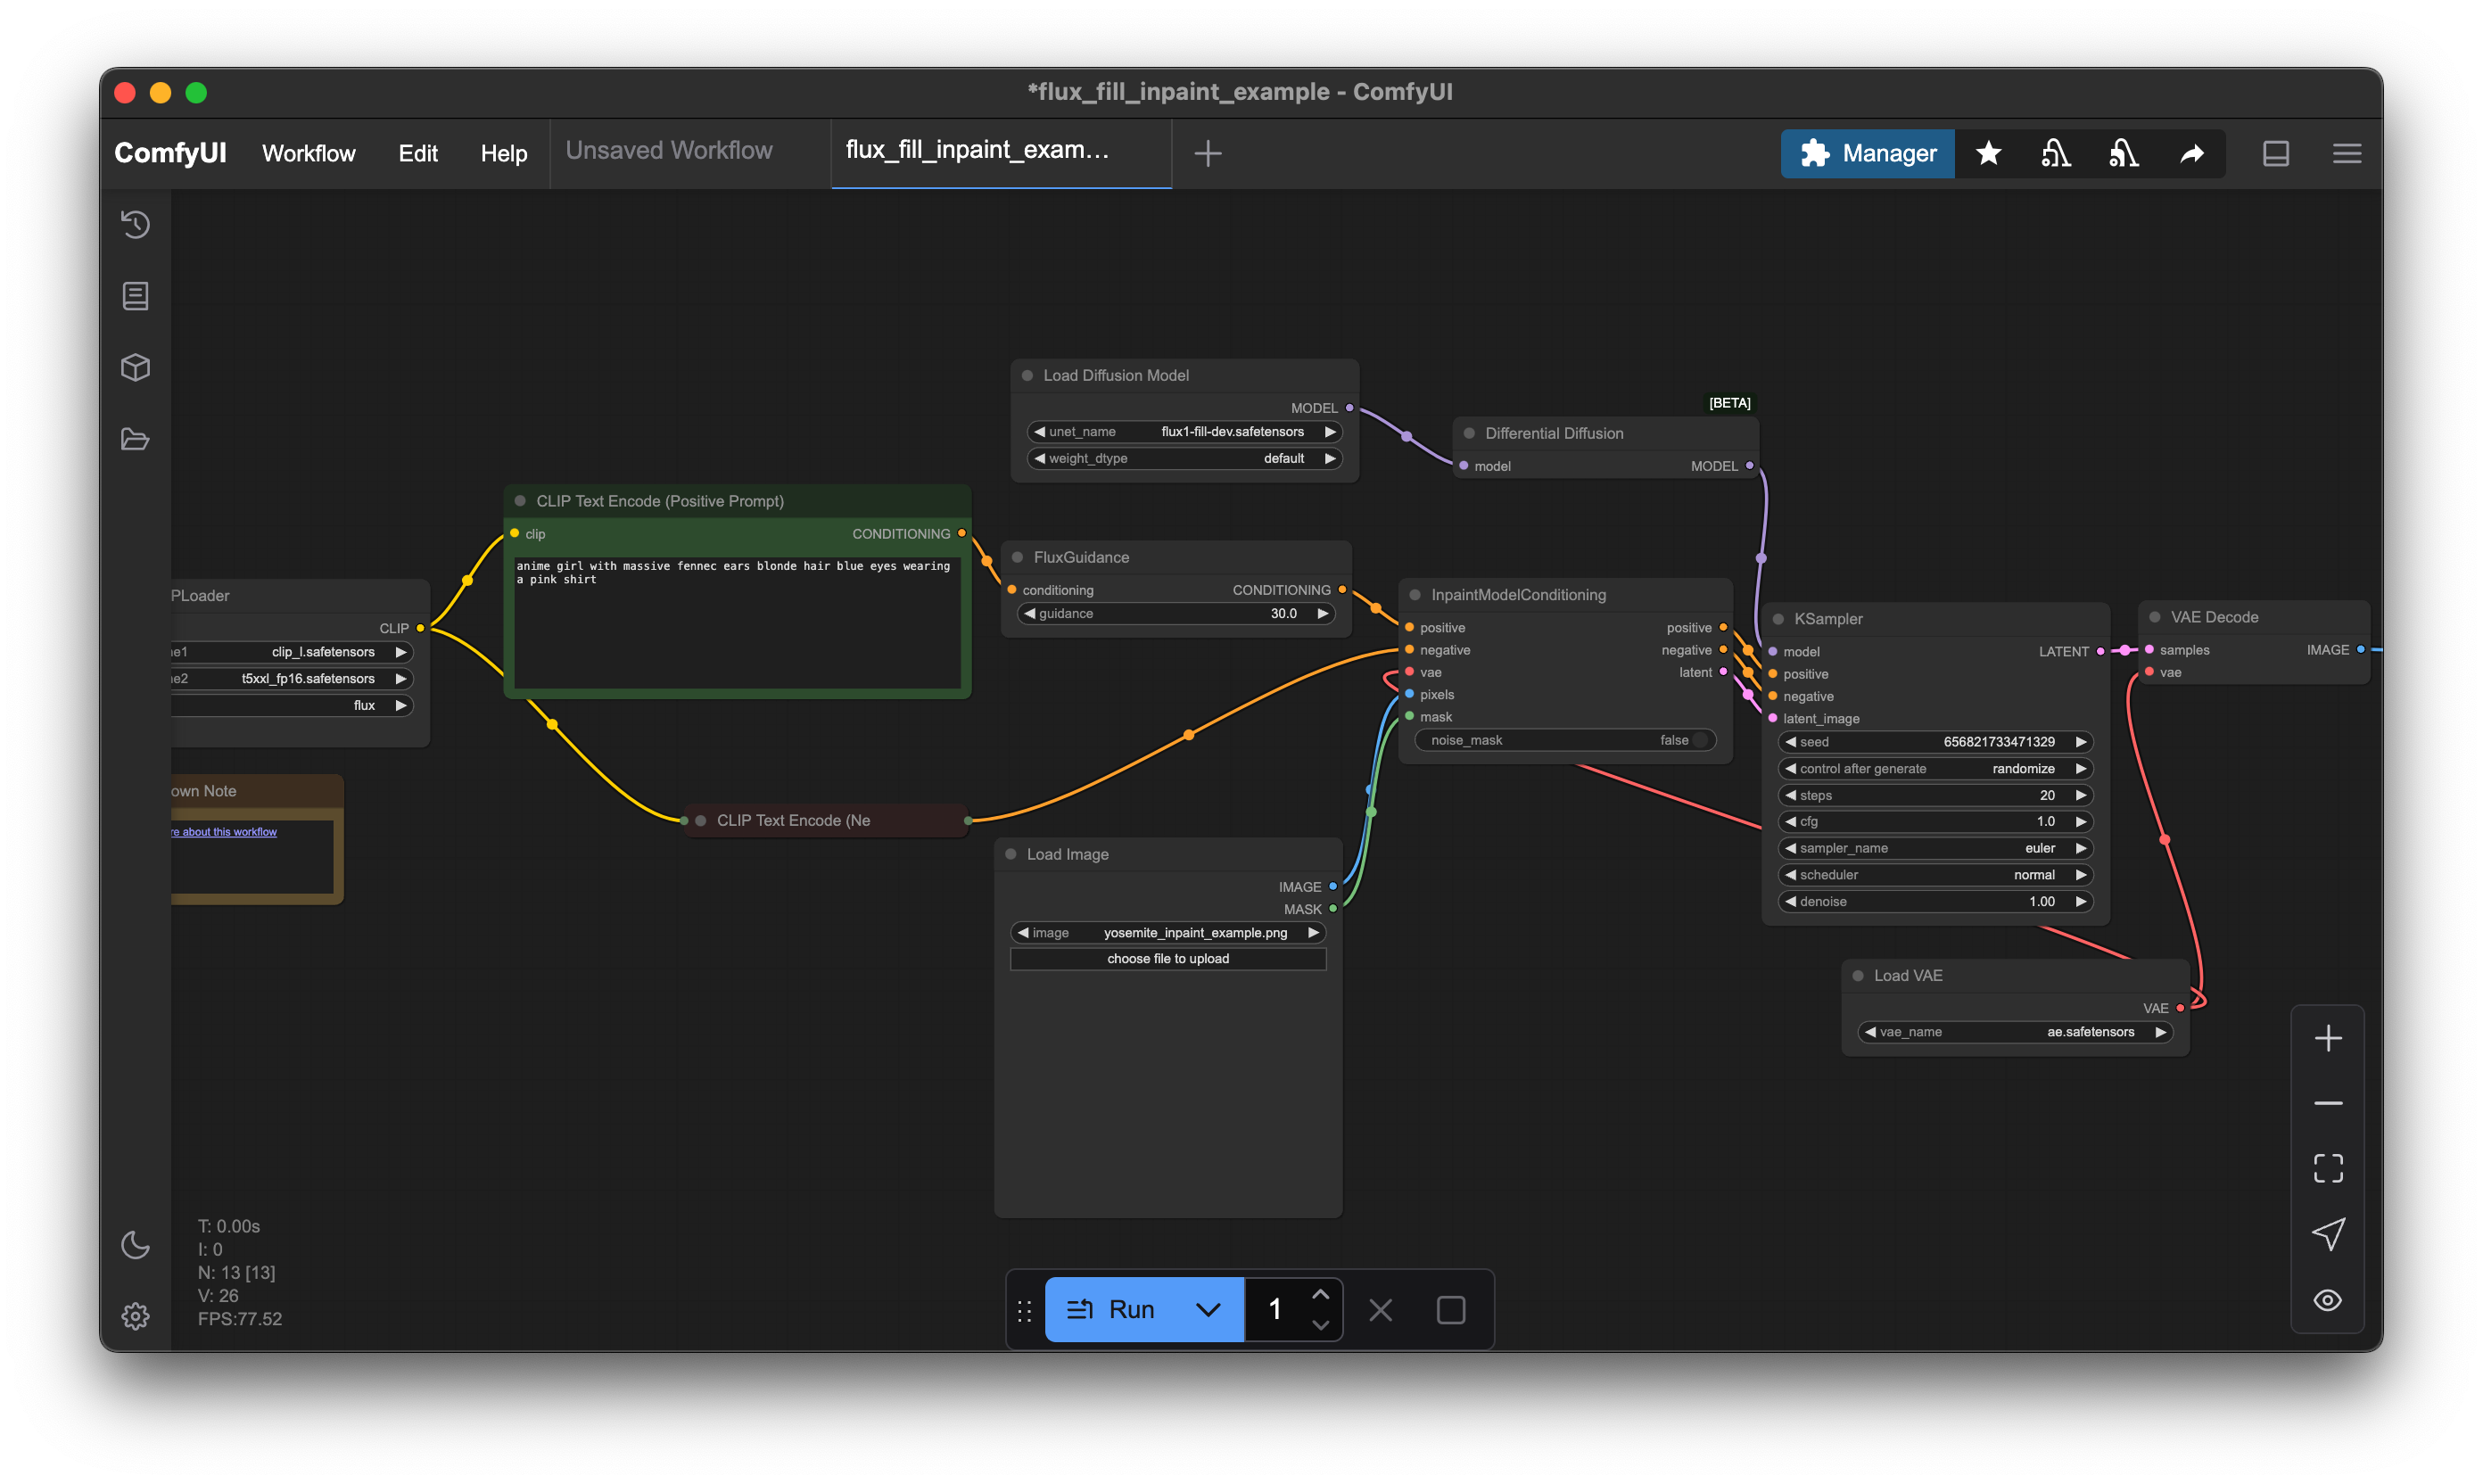
\includegraphics[width=0.8\textwidth]{./fig/set_param.png}
  \caption{参数调节}
  \label{fig:set_param}
\end{figure}

总的来说,目前初步容易上手的为使用文本去\red{生成海报的背景图片。}对于更精细化的图片生成,需要对图片生成有较深的了解,才能进行参数调节。以上的问题同样存在于视频生成领域。

\section{总结}
本文介绍了大型语言模型(LLM)的基本概念、国内主要AI厂商及其产品特点,以及实际应用案例。通过系统性梳理,我们可以得出以下几点结论:

\subsection{AI工具的发展现状}
大型语言模型已经从实验室技术发展为实用工具,国内形成了三大梯队的厂商格局:
\begin{itemize}
  \item \textcolor{red}{头部厂商}(百度、阿里、腾讯)拥有全面的技术能力和生态优势
  \item \textcolor{red}{垂直领域专家}(华为、商汤、科大讯飞)在特定行业展现出色表现
  \item \textcolor{red}{创新型公司}(DeepSeek、智谱AI等)在细分领域快速崛起
\end{itemize}

\subsection{AI工具的应用价值}
LLM在日常工作和学习中展现出多方面价值:
\begin{itemize}
  \item \textcolor{blue}{提升效率}:快速生成内容初稿,如文档、PPT、图片等
  \item \textcolor{blue}{辅助创意}:提供多角度思路,激发创新想法
  \item \textcolor{blue}{知识助手}:回答问题、解释概念、整合信息
  \item \textcolor{blue}{降低门槛}:使专业技能(如设计、编程)更易上手
\end{itemize}

\subsection{使用AI工具的最佳实践}
\begin{itemize}
  \item \textbf{确立明确目标}:清晰定义需求,提供足够详细的提示词
  \item \textbf{分步骤操作}:复杂任务拆解为小步骤,如先收集信息再生成内容
  \item \textbf{人机协作}:保持人工审核和调整,AI做加法,人做减法
  \item \textbf{迭代优化}:根据初步结果不断调整提示词,获取更理想输出
\end{itemize}

% % 添加参考文献
% \bibliographystyle{plain}
% \bibliography{references}

\end{document}
